\section{Methodology of Random Forest}

The sentiment analysis base on RF pipeline can be visually and logically described with the following flowchart:

\begin{figure}[ht]
    \centering
    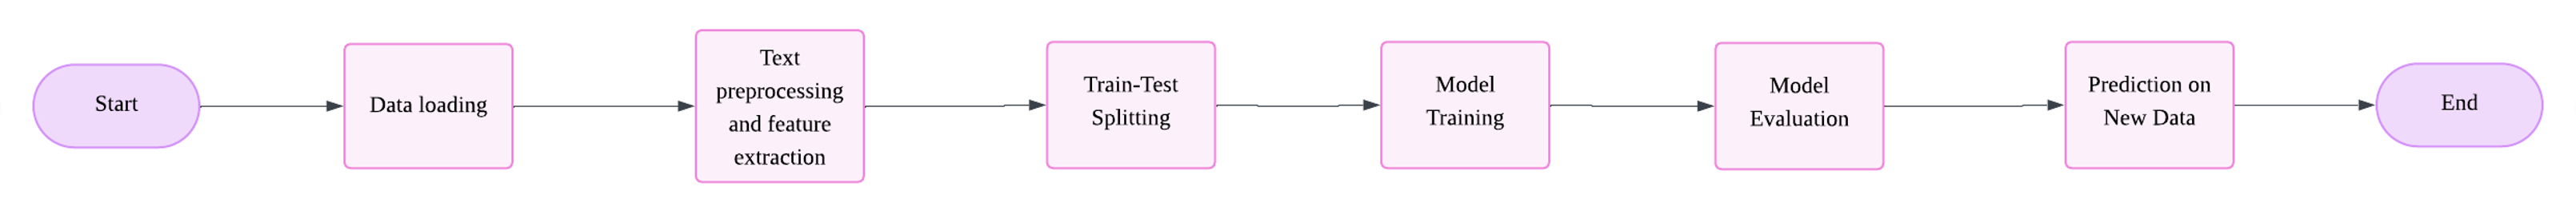
\includegraphics[width=1\textwidth]{pics/rf_steps.png}
    \caption{Random Forest analysis pipeline}
\end{figure}

\subsection{Step-by-step inputs and outputs}

\subsubsection*{Dataset Loading}
The first step is acquiring the dataset. We use the IMDB movie review dataset which is available on HuggingFace under the ID "stanfordnlp/imdb". The data is loaded using the "load\_dataset" function from HuggingFace's datasets library. After loading, it is converted into a pandas DataFrame to facilitate further processing.

Input: Dataset is fetched automatically.\\
Process: Dataset is downloaded and parsed.\\
Output: A structured dataset with two columns: text (the review) and label (the sentiment class).

\subsubsection*{Text Preprocessing and Feature Extraction}
Machine learning models cannot interpret raw textual data directly. Therefore, we must convert each review into a numerical representation. This is done using TF-IDF (Term Frequency-Inverse Document Frequency) vectorization.

TF-IDF calculates the importance of a word in a document relative to all other documents. We use the Tf-IDF Vectorizer from scikit-learn configured with "max\_features" as 10000 to limit vocabulary size and stop\_words as 'english' to remove commonly used words that carry little sentiment meaning.
This process transforms the review texts into a high-dimensional sparse matrix, where each row represents a review and each column represents a word feature.

Input: Raw review texts and labels.\\
Process: Tokenization, stopword removal and TF-IDF computation.\\
Output: A TF-IDF feature matrix X\_vec with shape.

\subsubsection*{Train-Test Splitting}
In this step, we split the dataset into training and testing subsets using scikit-learn's "train\_test\_split" function. We allocate 80\% of the data to training and 20\% to testing. The split is randomized but reproducible due to a fixed random seed by setting "random\_state" as 42.
This step ensures that the model is trained on one portion of the data and evaluated on completely unseen data, which simulates a real-world deployment scenario.

Input: TF-IDF feature matrix X\_vec and label vector y. \\
Process: Random partitioning of data into training and test sets. \\
Output: X\_train and y\_train used to train the model, X\_test and y\_test used to evaluate the model.

\subsubsection*{Model Training}
We train a Random Forest Classifier which is an ensemble learning algorithm. It creates multiple decision trees and combines their predictions to improve accuracy and reduce overfitting.
The classifier is instantiated using scikit-learn's RandomForestClassifier. For the initial experiment, we use default settings with "n\_estimators" as 100, which means 100 decision trees are built.
The training data (X\_train and y\_train) is fed into the "fit" function, which constructs the trees by learning patterns in the TF-IDF features that differentiate positive and negative reviews.

Input: X\_train (TF-IDF vectors) and y\_train (labels). \\
Process: Each tree learns decision rules from data subsets and the forest aggregates these decisions.\\
Output: A trained RandomForestClassifier model object.

\subsubsection*{Model Evaluation}
After training, we evaluate the model's ability to classify reviews it has never seen before. This is done using the test set (X\_test, y\_test).
We use the "predict" method to generate predicted labels and then calculate performance metrics. These metrics help understand both overall accuracy and error distribution which is especially important in binary classification tasks.

\begin{itemize}
    \item Accuracy: the proportion of correct predictions
    \item Classification Report: includes precision, recall and F1-score
    \item Confusion Matrix: shows how many true/false positives and negatives the model predicted
\end{itemize}

Input: Trained model, X\_test and y\_test. \\
Process: Predict labels and compare against true values \\
Output: Accuracy score, detailed classification report and confusion matrix.

\subsubsection*{Prediction on New Data}
Finally, the trained model can be used to predict sentiment on new movie reviews provided by users. Before prediction, the new review text must go through the same TF-IDF transformation as the training data.
The "vectorizer.transform" method is used to convert raw text to a vector which is then passed to the model's "predict" method.

Input: New review text. \\
Process: Apply TF-IDF vectorization, ten make prediction. \\
Output: A sentiment prediction 0 (negative) or 1 (positive).


\subsection{Implementation of Random forest}
The implementation of this sentiment analysis project is fully contained, which consists of the following key components.

\begin{enumerate}
    \item Loading the IMDB Dataset from HuggingFace: The script uses the datasets library to automatically fetch the standfordnlp/imdb dataset. Only the labeled train and test splits are used. The data is then converted into pandas DataFrames for ease of manipulation and preprocessing.
    \item TF-IDF Vectorization: The text data is transformed into numerical features using TF-IDF Vectorizer from scikit-learn. The vectorizer is configured with max\_features as 10000 and stop\_words as 'english' to ensure a compact, meaningful vocabulary. This transforms raw text into a sparse matrix of features suitable for machine learning.
    \item Model Training and Prediction Using Random Forest: A RandomForestClassifier is initialized with 100 decision trees. The classifier is trained on the training set and then tested to obtain the sentiment predictions on the test data.
    \item Evaluation Metrics Output: After prediction, the script computes accuracy score, confusion matrix, classification report including precision, recall and F1-score. These metrics provide a comprehensive view of how well the model performs on unseen data.
    \item Confusion Matrix Visualization and Saving: The confusion matrix is plotted as a heatmap for better readability and visual analysis. The resulting plot is saved as an image file.
\end{enumerate}


\subsection{Results of random forest}
In this section, we present the experimental results obtained from training and evaluating the Random Forest classifier on the IMDB movie review dataset. The results are discussed in terms of standard classification metrics including accuracy, precision, recall, F1-score and confusion matrix.
After training the model on the preprocessed TF-IDF features and evaluating it on the unseen test set, the model achieved accuracy: 85.3\%. This shows that the Random Forest model is able to correctly classify the sentiment of about 8.5 out of every 10 reviews. Given the simplicity of the feature representation, this is a strong baseline.

\subsubsection*{Classification Report}
\begin{figure}[ht]
    \centering
    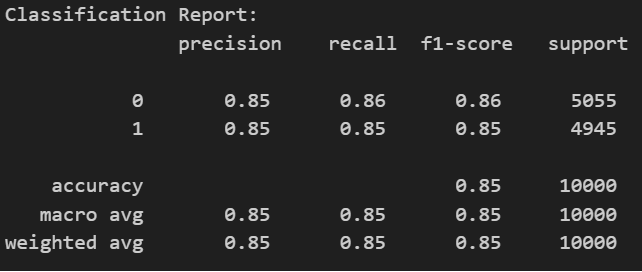
\includegraphics[width=0.5\textwidth]{pics/rf_eval_report.png}
    \caption{Classification Report of Random Forest}
\end{figure}

Precision: When the model predicts a sentiment, it is correct about 85\% of the time.
Recall: The model is slightly lower at identifying positive reviews than negative ones.
F1-score: A good balance between precision and recall, indicating consistent performance.

\subsubsection*{Confusion Matrix}
This confusion matrix shows the number of true/false predictions made by the classifier:

\begin{figure}[ht]
    \centering
    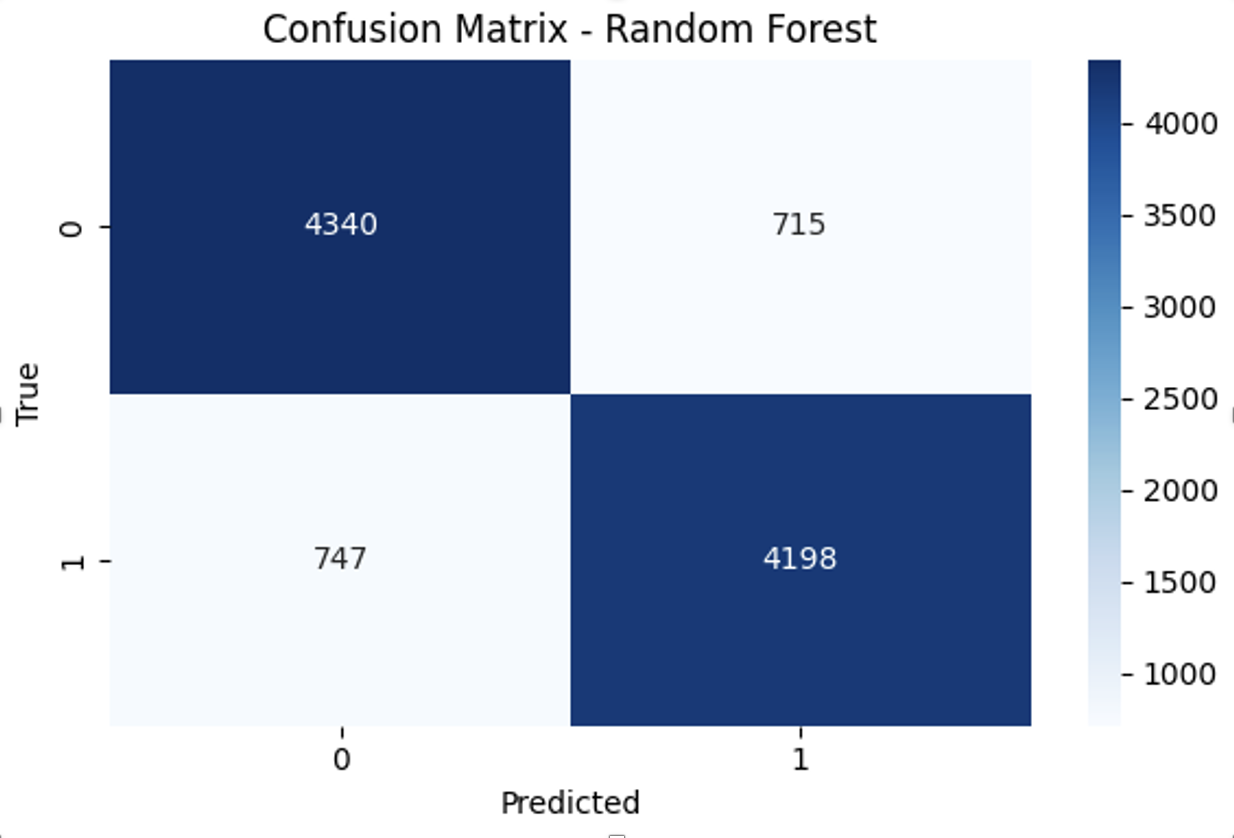
\includegraphics[width=0.4\textwidth]{pics/rf_eval_metrix.png}
    \caption{Confusion Matrix of Random Forest}
\end{figure}

Interpretation:
True Negatives (TN): 4340 —— correctly predicted negative reviews.
False Positives (FP): 715 —— negative reviews incorrectly predicted as positive.
False Negatives (FN): 747 —— positive reviews incorrectly predicted as negative.
True Positives (TP): 4198 —— correctly predicted positive reviews.

\subsubsection*{Conclusion}
Random Forest proves to be a reliable and interpretable model for sentiment analysis of movie reviews. While deep learning methods may offer marginal gains, ensemble methods like Random Forest offer a good balance between performance and computational efficiency.


